\section{Diagramme général des cas d'utilisation UML}

\subsection{Principes de lecture du diagramme}

Le diagramme général des cas d'utilisation présenté en figure \ref{fig:uc_general} constitue le livrable central de modélisation de cette étude préliminaire. Il a été conçu au format natif Draw.io (\texttt{diagrammes/cas-utilisation-general.drawio}) dans le strict respect de la notation UML 2.5 :

\begin{itemize}
  \item \textbf{Frontière du système :} le cadre principal délimite le périmètre de l'application (\emph{Système de suivi des dépenses budgétaires}) et le sépare des cinq acteurs externes au logiciel.
  \item \textbf{Positionnement des acteurs :} les acteurs à l'initiative des demandes et des prestations (\emph{Ordonnateur} et \emph{Fournisseur}) sont placés à gauche du système ; les acteurs chargés du contrôle budgétaire, de la réception matière et de la prise en charge comptable (\emph{Contrôleur financier}, \emph{Comptable matière}, \emph{Comptable public}) sont placés à droite.
  \item \textbf{Structuration interne :} quatre cadres en pointillés regroupent les dix-neuf cas d'utilisation par grands domaines fonctionnels afin de préserver la lisibilité de l'ensemble.
  \item \textbf{Associations et dépendances :} les traits continus représentent la participation d'un acteur à un cas d'utilisation ; les flèches pointillées ouvertes portent les stéréotypes normalisés \texttt{« include »} (inclusion obligatoire) et \texttt{« extend »} (extension conditionnelle).
\end{itemize}

\begin{landscape}
\begin{figure}[H]
\centering
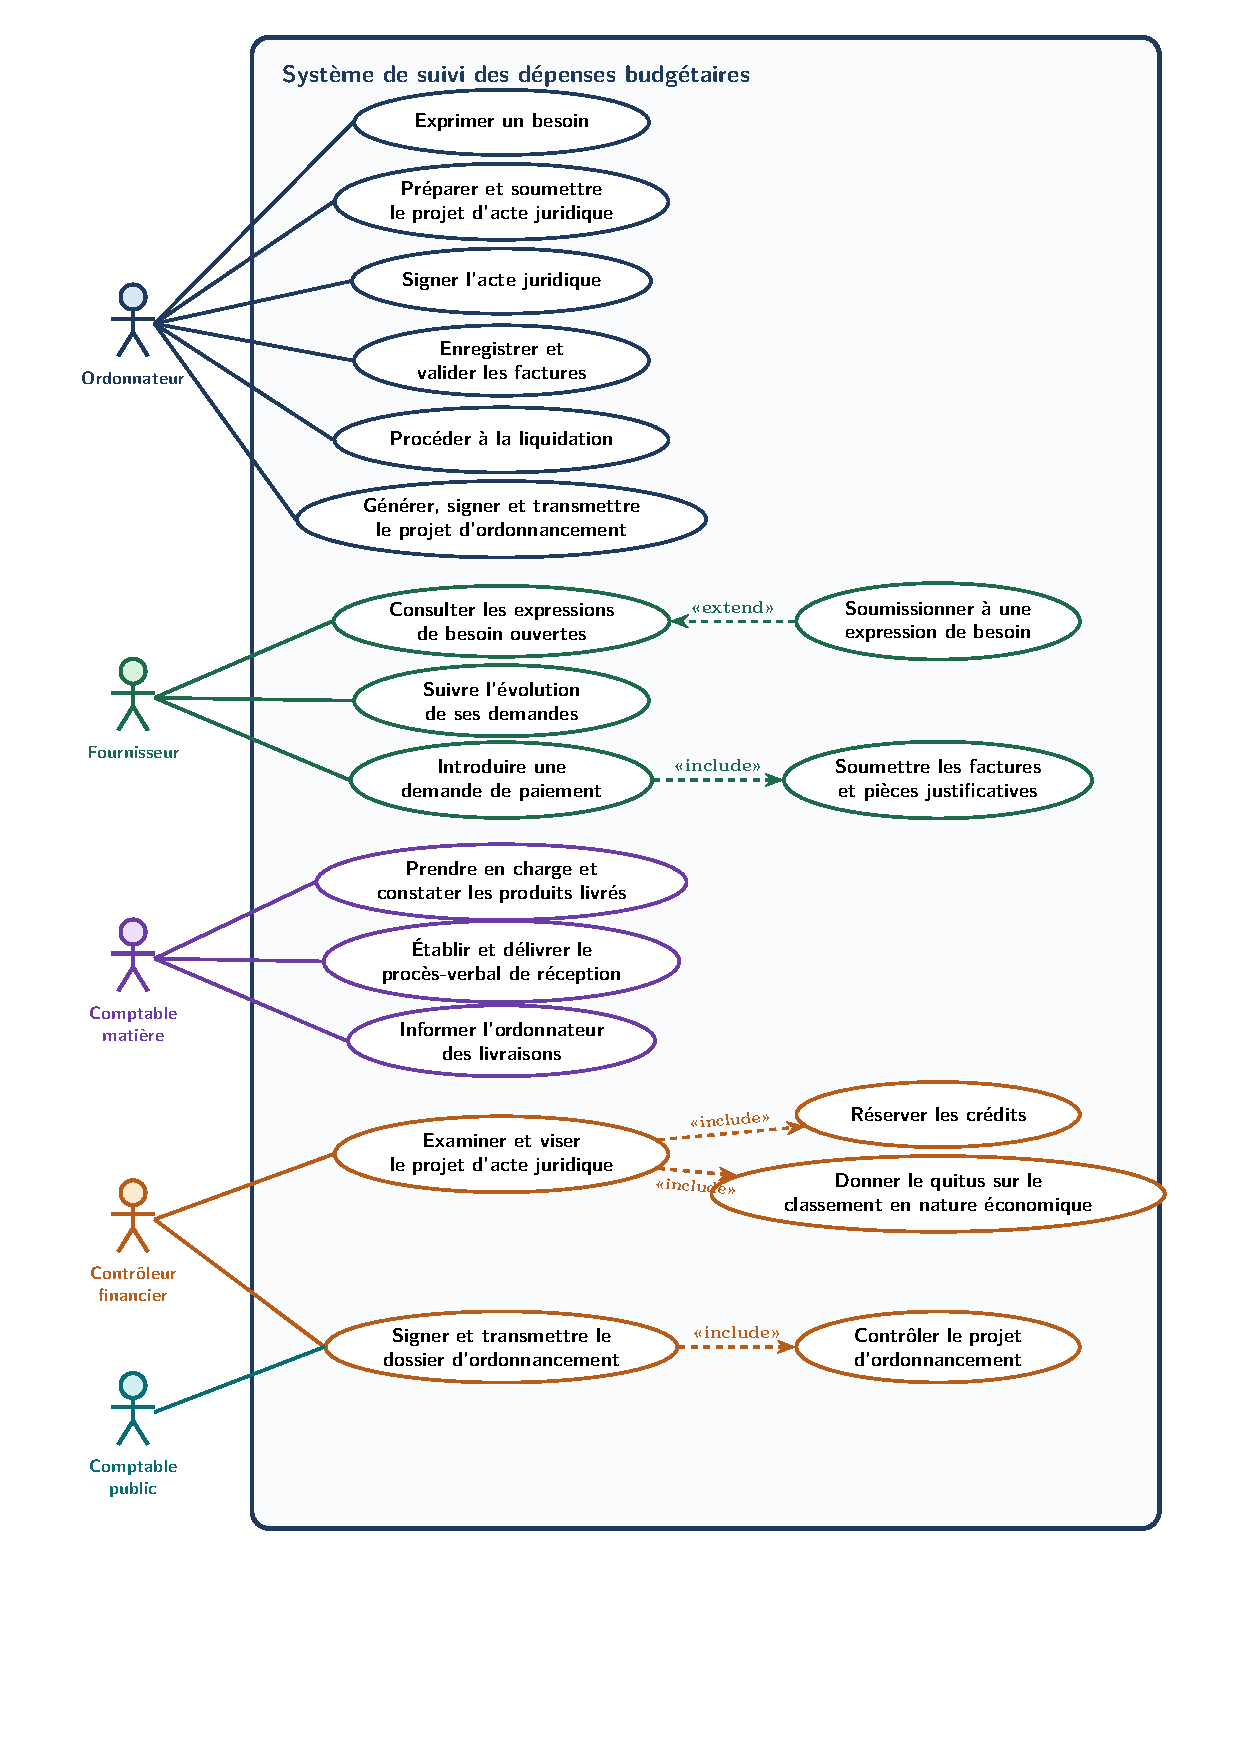
\includegraphics[width=0.98\linewidth,height=0.82\textheight,keepaspectratio]{../diagrammes/cas-utilisation-general.pdf}
\caption{Diagramme général des cas d'utilisation UML — Système de suivi des dépenses budgétaires (fichier source : \texttt{diagrammes/cas-utilisation-general.drawio})}
\label{fig:uc_general}
\end{figure}
\end{landscape}
